\begin{figure}[ht] 
 	\centering 
 	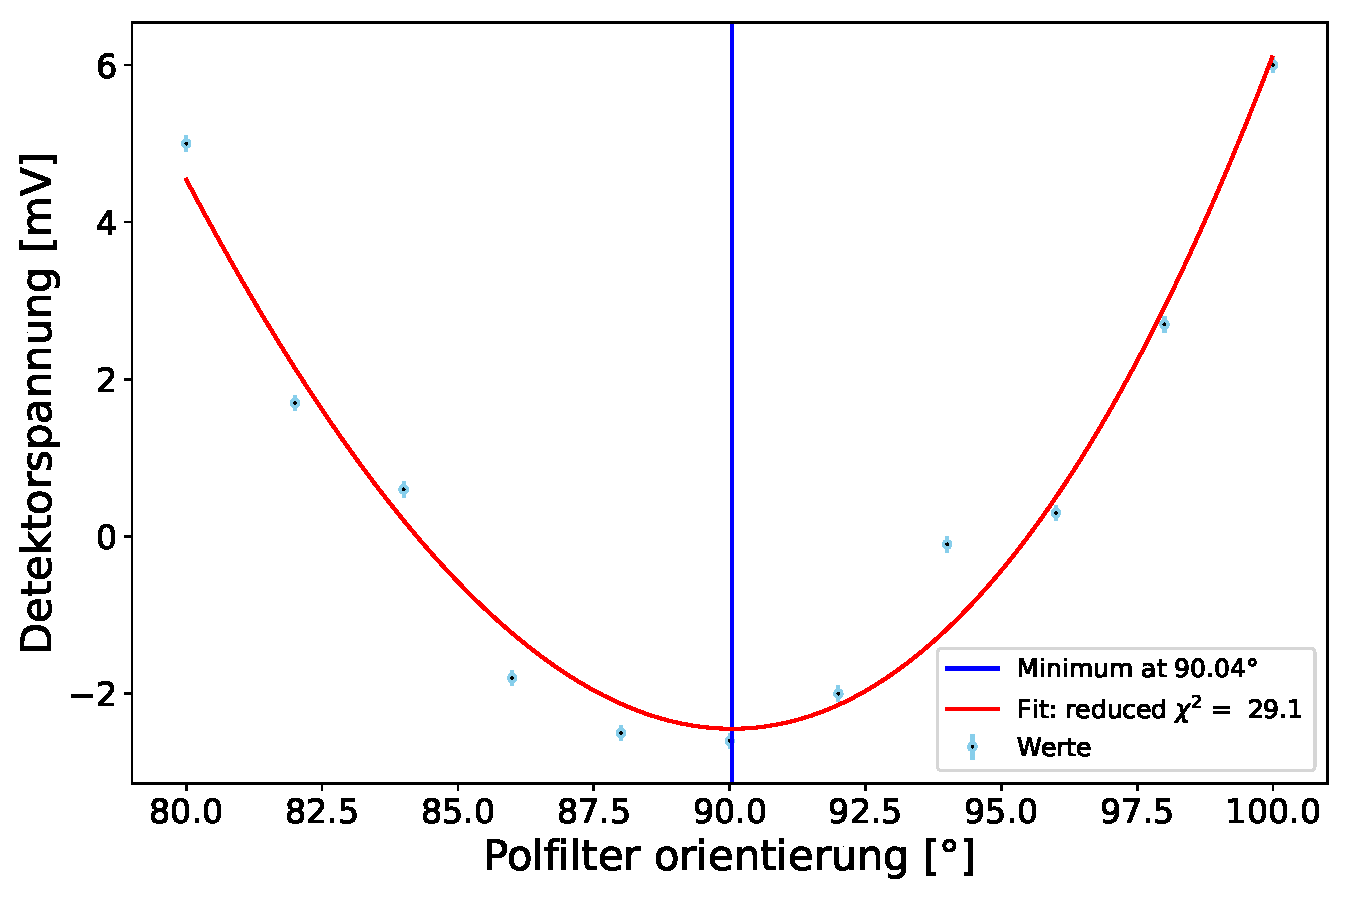
\includegraphics[width= 0.65 \textwidth]{Fits/pol_offset_Fit.pdf} 
	\caption{pol offset, Fit} 
 	\label{fig:pol offset, Fit} 
\end{figure}
 
\begin{align} 
 	 f(x) = a x^{4} + b x^{2} + c
\end{align} 

 
\begin{table}[ht] 
	\centering 
	\caption{pol offset, Fit Parameter Tabelle} 
	\label{tab: pol offset, Fit Parameter Tabelle}
	\begin{tabular}{|l|c|}
		\hline
		Parameter Name	&	Wert \\ \hline
		a	&	 2e-06. $\pm$  1e-07.\\ \hline
		b	&	-0.0388 $\pm$  0.002\\ \hline
		c	&	 155.0 $\pm$  9.4\\ \hline
	\end{tabular} 
\end{table}
 
\begin{table}[ht] 
	\centering 
	\caption{pol offset, Messwerte Tabelle} 
	\label{tab: pol offset, Messwerte Tabelle}
	\begin{tabular}{|c|c|}
		\hline
		Polfilter orientierung [°] 	&	 Detektorspannung [mV]\\ \hline
		80.0 $\pm$ 0.2 	&	 5.0 $\pm$ 0.1 \\ \hline
		82.0 $\pm$ 0.2 	&	 1.7 $\pm$ 0.1 \\ \hline
		84.0 $\pm$ 0.2 	&	 0.6 $\pm$ 0.1 \\ \hline
		86.0 $\pm$ 0.2 	&	 -1.8 $\pm$ 0.1 \\ \hline
		88.0 $\pm$ 0.2 	&	 -2.5 $\pm$ 0.1 \\ \hline
		90.0 $\pm$ 0.2 	&	 -2.6 $\pm$ 0.1 \\ \hline
		92.0 $\pm$ 0.2 	&	 -2.0 $\pm$ 0.1 \\ \hline
		94.0 $\pm$ 0.2 	&	 -0.1 $\pm$ 0.1 \\ \hline
		96.0 $\pm$ 0.2 	&	 0.3 $\pm$ 0.1 \\ \hline
		98.0 $\pm$ 0.2 	&	 2.7 $\pm$ 0.1 \\ \hline
		100.0 $\pm$ 0.2 	&	 6.0 $\pm$ 0.1 \\ \hline
	\end{tabular} 
\end{table}
 
